\chapter{\acrlong{EAC}}
\label{chapter:eac}

Los métodos de clustering ensambles se basan en tomar resultados generados por múltiples algoritmos de clustering y llegar a un consenso que sea más correcto que los resultados individuales de los algoritmos utilizados. Uno de estos métodos, que utilizaremos en este capítulo, es \gls{EAC} \citep{fred2005combining}.

Sea $X = {x_1, x_2,...,x_n}$ nuestro conjunto de datos donde $x_i \in R^d$ y $R^d$ es un espacio de $d$ features. Luego, utilizando un método de clustering especifico se obtiene una partición $P$ la cual encuentra $k$ clusters en el conjunto mencionado. Dado $N$ algoritmos de clustering podemos entonces derivar $N$ particiones $P$ las cuales definen los clusters encontrados por cada algoritmo. Por último, definimos al conjunto de estas particiones como:

\begin{equation}
\mathbb{P} = \{P^1, P^2,...,P^N\}
\end{equation}

\begin{multline}
\hfill
    \begin{split}
    P^1 = \{C^1_1, C^1_2,...,C^1_{k_1}\}
    \end{split} \hfill \break
\hdots \hfill \break
    \begin{split}
    P^N = \{C^N_1, C^N_2,...,C^N_{k_N}\}
    \end{split}
\hfill
\end{multline}

\noindent donde $C^i_j$ es el cluster $j$th en la partición $P^i$, la cual tiene $k_i$ clusters. Además, dado $n^i_j$ como la cardinalidad de $C^i_j$, se cumple que $\sum_{j=1}^{k_i} n^i_j=n, \ \ i=1,...,N$.

Utilizando la información disponible en las $N$ particiones de nuestros datos en $\mathbb{P}$, el objetivo de \gls{EAC} es obtener una partición de datos ``óptima'' llamada $P^*$. Adicionalmente, definimos $k^*$ como el número de clusters en $P^*$.

Idealmente, $P^*$ debe cumplir con las siguientes propiedades:
\begin{enumerate}
    \item Consistencia con el ensamble de clusterings $\mathbb{P}$: Significa que $P^*$ sea el resultado de un acuerdo entre las diferentes partes encontradas $P^i, i=1,...,N$.
    \item Robustez antes pequeñas variaciones en $\mathbb{P}$: Los cantidad de clusters y los puntos pertenecientes a cada cluster en $P^*$ deberían ser invariantes ante pequeñas perturbaciones de $\mathbb{P}$.
    \item Ajuste con respecto al \gls{GT}: Los clusters encontrados deberán coincidir fuertemente con las verdaderas etiquetas de nuestros datos.
\end{enumerate}

La idea detrás de \gls{EAC} es combinar los resultados de múltiples clusterings en una única partición de datos, interpretando cada uno de estos resultados como una ``evidencia independiente'' de la organización de los datos, como puede apreciarse en la Fig~\ref{fig:eac-example}. Esto nos requiere abordar los siguientes tres problemas, que definen cada etapa del algoritmo de \gls{EAC}:

\begin{figure}
    \centering
    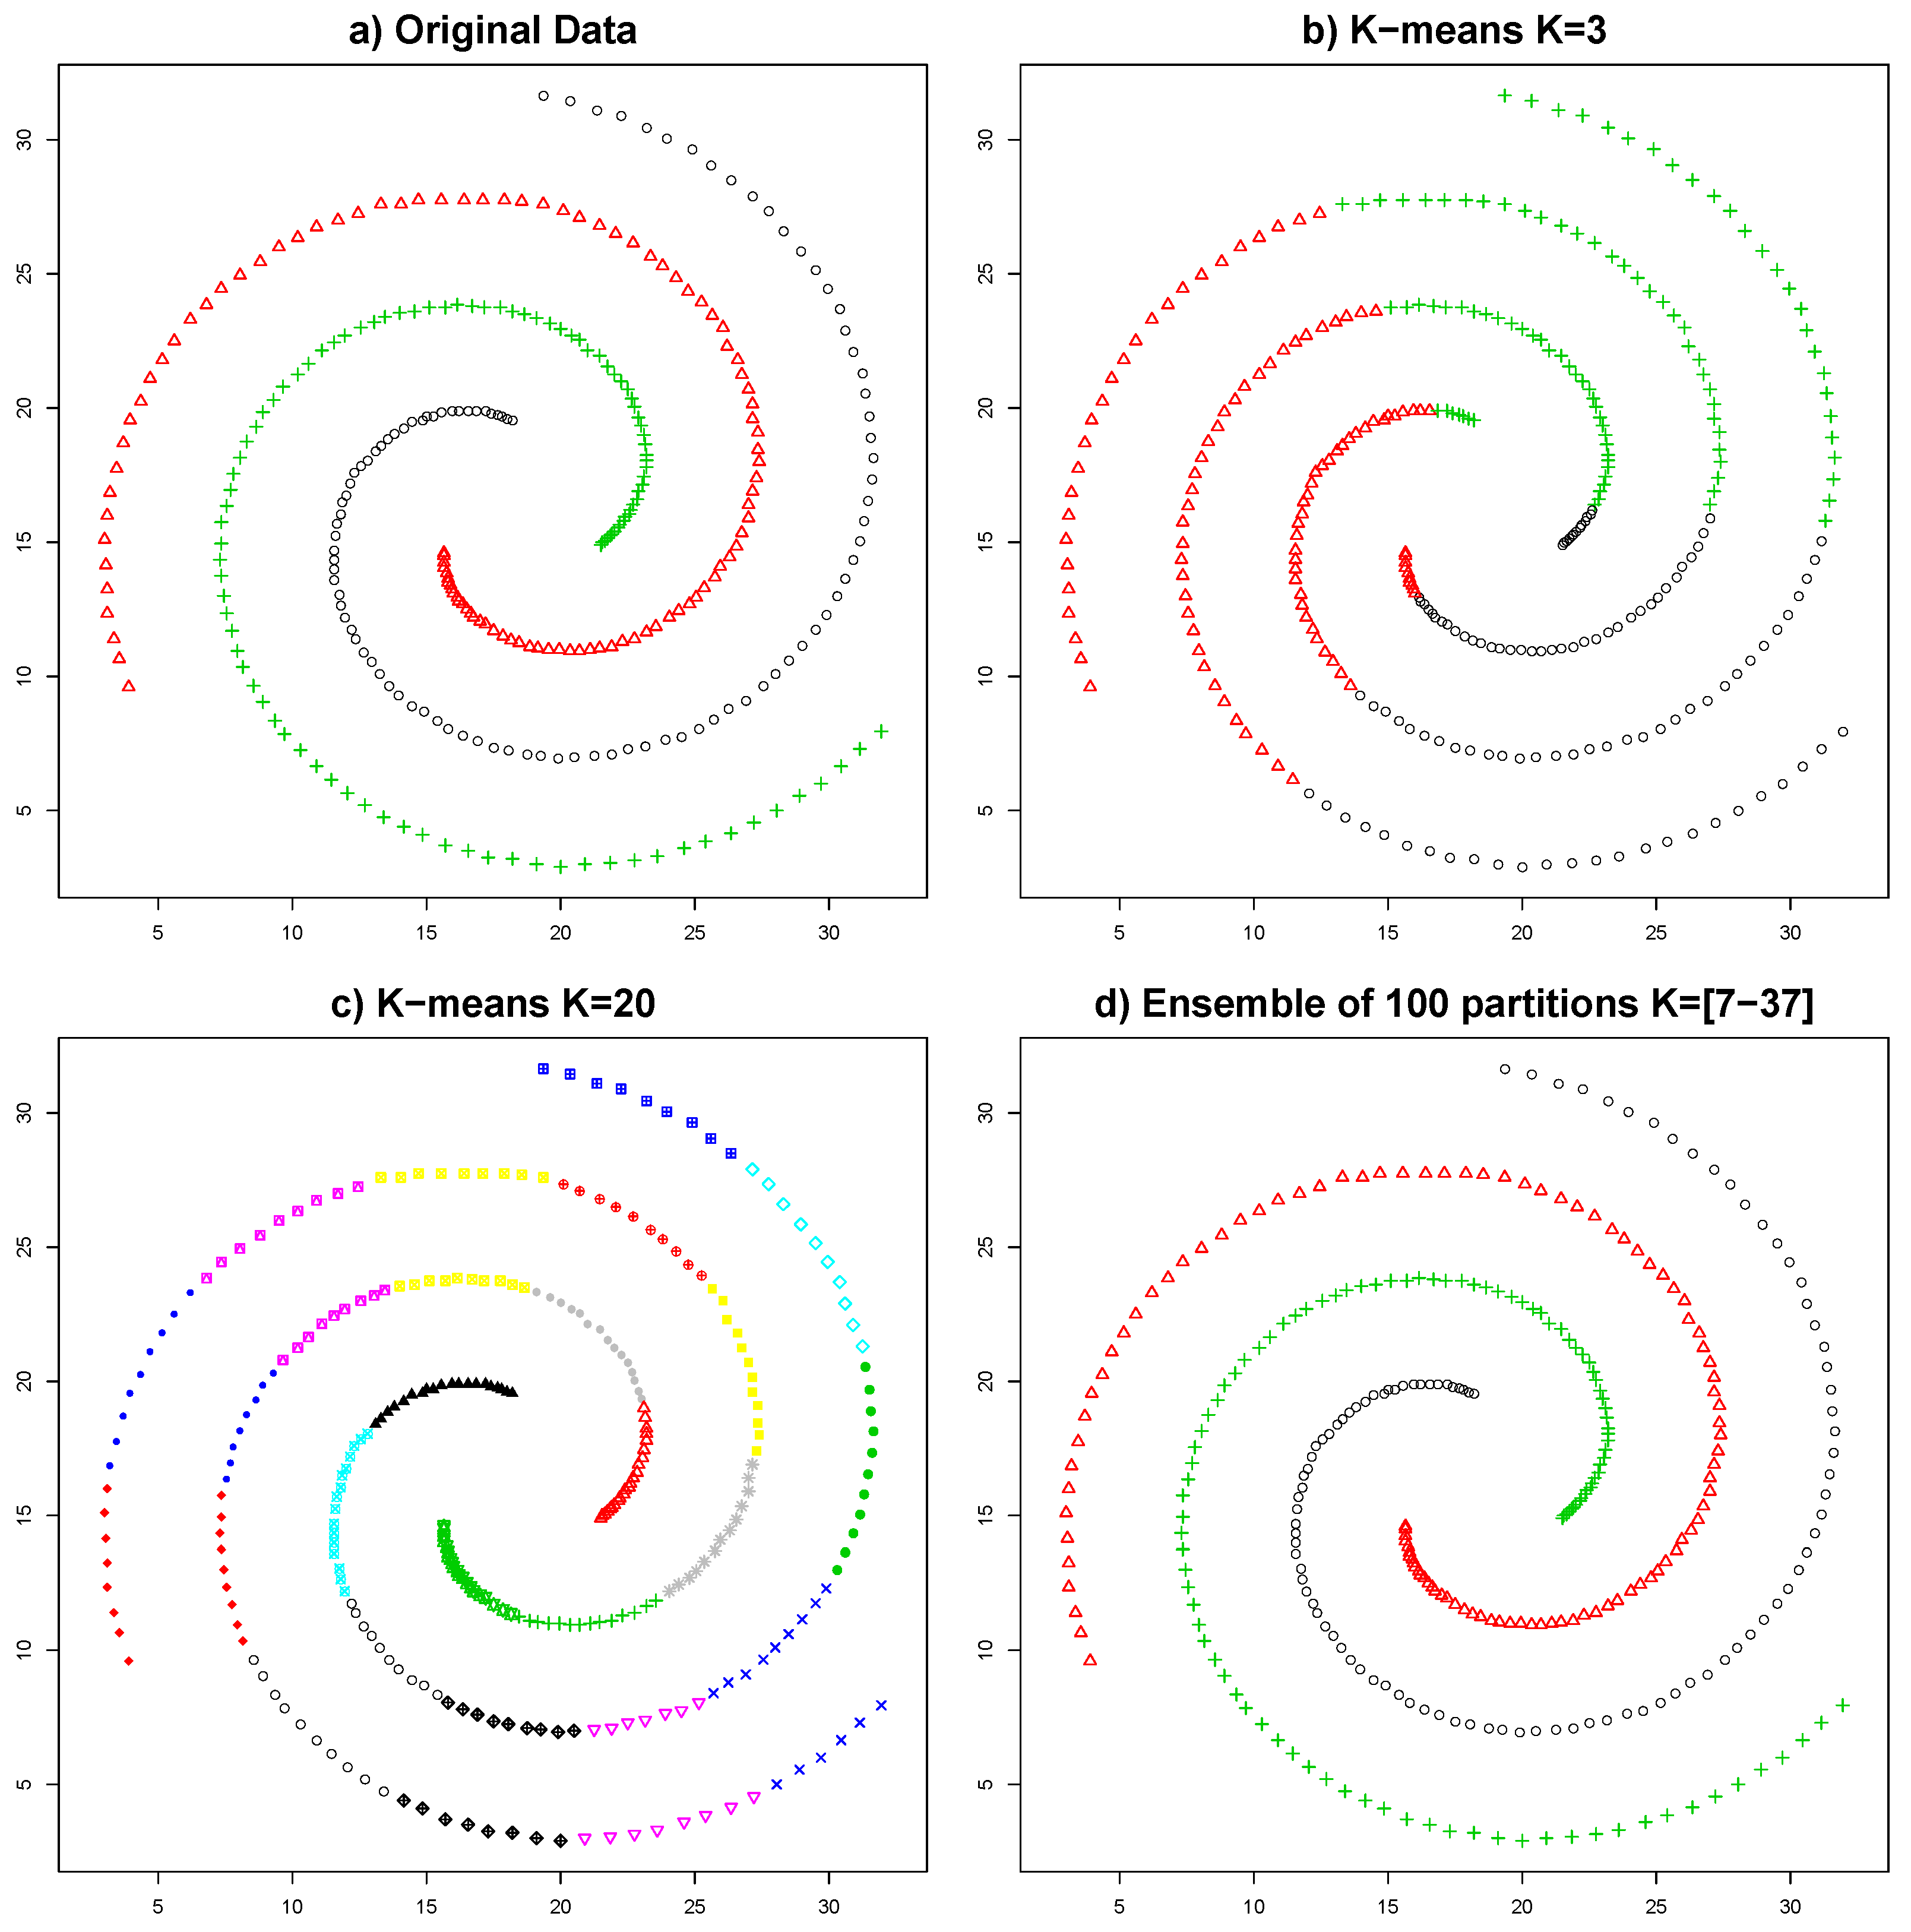
\includegraphics[width=.9\textwidth]{evidence accumulation clustering/figures/ensamble-example.png}
    \caption{Comparación de clustering aplicado a un dataset entre diferentes corridas de k-means contra \gls{EAC} con 100 instancias de k-means. Variando la cantidad de clusters buscados por estos entre 7 y 37 \citep{marquez2019positive}.}
    \label{fig:eac-example}
\end{figure}

\begin{enumerate}
    \item  Cómo generamos el ensamble de particiones.
    \item  Cómo combinamos la evidencia.
    \item  Cómo extraemos una partición de datos (conjunto de clusters) consistente de la evidencia combinada.
\end{enumerate}

Hay diferentes formas de abordar el primer problema, las cuales pueden separarse de las siguientes categorías:

\begin{enumerate}
\item Elección de representación de datos:
    \begin{enumerate}
     \item Empleando diferentes métodos de preprocesamiento y/o extracción de features, lo que resulta en diferentes representaciones de los datos o espacio de features.
     \item Explorando subespacios de la misma representación de datos.
     \item Perturbando los datos con métodos de bootstrapping o sampling.
     \end{enumerate}
\item Elección de algoritmos de clustering o parámetros de los algoritmos:
    \begin{enumerate}
     \item Aplicando diferentes algoritmos de clustering.
     \item \label{chosen-variation} Usando el mismo algoritmo pero con diferentes parámetros o inicializaciones.
     \item Explorando diferentes medidas de disimilitud para evaluar relaciones en nuestros datos.
     \end{enumerate}
\end{enumerate}

En este trabajo nos interesara aplicar lo mencionado en \ref{chosen-variation}. Es decir, utilizaremos un algoritmo en particular, k-means, múltiples veces con semillas diferentes para generar el ensamble de clusters.

El método de clustering k-means \citep{macqueen1967some} es un algoritmo clásico del área de minería de datos. Este propone, dado un conjunto de k clusters buscados, asignar de forma aleatoria los centros de dichos clusters e iterativamente optimizarlos, asignando los puntos al centro del cluster más cercano en cada iteración. Como el algoritmo es naturalmente inestable significa que podemos utilizar la variabilidad de múltiples corridas de k-means para llegar a un consenso, como se propone realizar con \gls{EAC}.

Cabe aclarar que \gls{EAC} no asume el número de clusters $k_i$ para cada partición obtenida $P^i$, por lo que cada $k_i$ pueden ser no sólo diferentes al número de clusters buscado por \gls{EAC}, sino que también entre sí.

Una vez obtenido el ensamble de particiones, pasaremos a combinar la información proveída de estos con una matriz de co-asociación como puede observarse en la Fig~\ref{fig:co-association-matrix}, la cual nos permitirá relacionar la información obtenida con cada partición incluso si la cardinalidad varía entre ellas. Dicha matriz, también llamada matriz de similitud, es de dimensión $n \times n$ y representa qué tan similares son los objetos de un conjunto entre sí (en nuestro caso, los puntos de nuestros datos), asignándole un valor de cero a uno a cada una de sus celdas.

El algoritmo propone un mecanismo de votación que será utilizado como métrica de similitud entre los puntos de nuestros datos, bajo la suposición de que dos puntos pertenecen al mismo cluster si se encontraron en el mismo cluster repetidas veces en el ensamble de particiones. Dicha métrica es la siguiente:

$$
C(i,j) = \frac{n_{ij}}{N},
$$

\noindent donde $n_{ij}$ es el número de veces que el par de puntos $(i,j)$ son asignados al mismo cluster en las $N$ particiones. Por lo cual, asignaremos el valor de $C(i,j)$ a la celda de la matriz de similitud de la fila $i$ y la columna $j$.

\begin{figure}
    \centering
    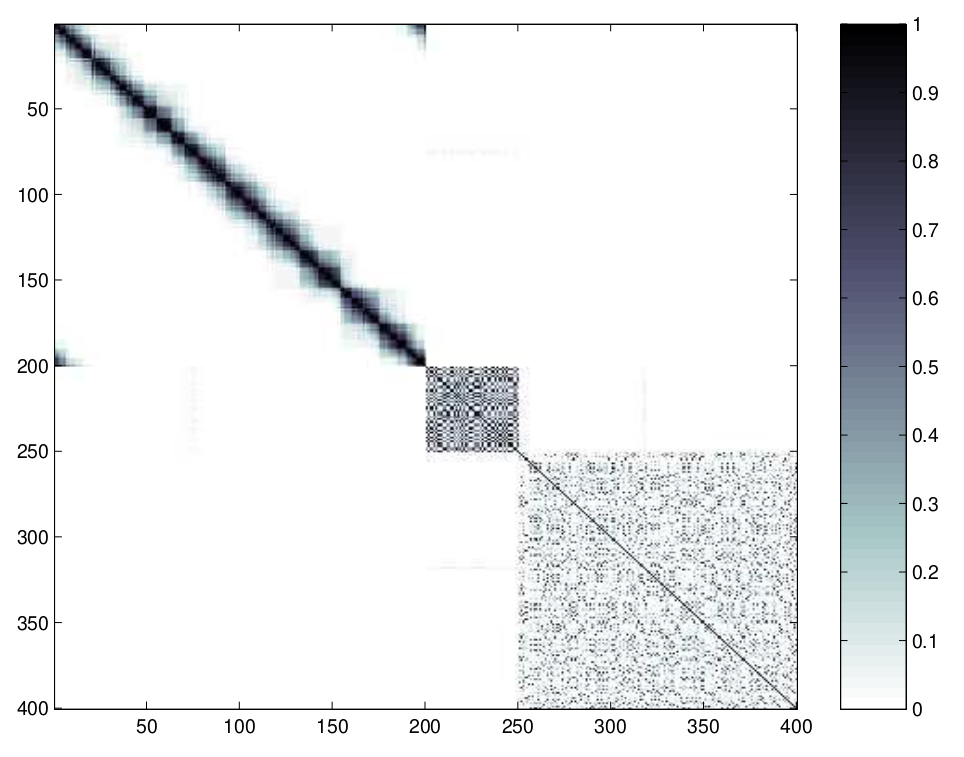
\includegraphics[width=.9\textwidth]{evidence accumulation clustering/figures/co-association matrix.png}
    \caption{Matriz de asociación obtenida con \gls{EAC} \citep{fred2005combining}, en donde ambos ejes representan puntos en un conjunto de datos, y cada celda que tan similares son estos entre ellos. Con los valores más altos indicando mayor similitud.}
    \label{fig:co-association-matrix}
\end{figure}

Una vez generada la matriz de similitud podemos aplicar cualquier algoritmo de clustering sobre ésta. \citet{fred2005combining} optan por utilizar clustering jerárquico aglomerativo con single o average linkage.

Para correr dicho algoritmo en este trabajo utilizaremos la implementación realizada por la librería de Python ``combo''\footnote{Fue necesario crear un fork de la librería para poder solucionar un bug y realizar optimizaciones generales de la memoria utilizada por su implementación de \gls{EAC}, como así optimizaciones extra específicas para nuestro campo de estudio. Se puede encontrar en \href{https://github.com/originalnicodr/combo}{https://github.com/originalnicodr/combo}.} \citep{zhao2020combo}. Aunque el paper original describe cómo la elección de donde cortar el dendrograma se realiza a partir de una medida de ``tiempo'' respecto a qué tanto se mantienen los clusters en el dendrograma antes de juntarse con otro, la librería mencionada nos da la opción de cortar el dendrograma en donde queramos para así obtener una partición de nuestros datos con la cantidad específica de clusters que buscamos. Esto nos es de especial utilidad para realizar los experimentos y comparaciones que venimos haciendo en los capítulos anteriores.

\section{Detección de dos componentes: Disco y esferoide}

En este trabajo utilizamos el algoritmo descrito de \gls{EAC} con \gls{HC} y single linkage. El algoritmo que decidimos utilizar fue k-means con $k_i = 100, i = 1, ..., N$.

Aunque comenzamos utilizando $N = 500$ k-means con inicializaciones al azar, el costo computacional de \gls{EAC} es tan grande para nuestro espacio de datos que nos vimos obligados a utilizar $N=100$ en su lugar, con los resultados variando poco entre ellos como se puede observar en la Fig~\ref{fig:eac-amount-kmeans-comparison}


\begin{figure}
    \centering
    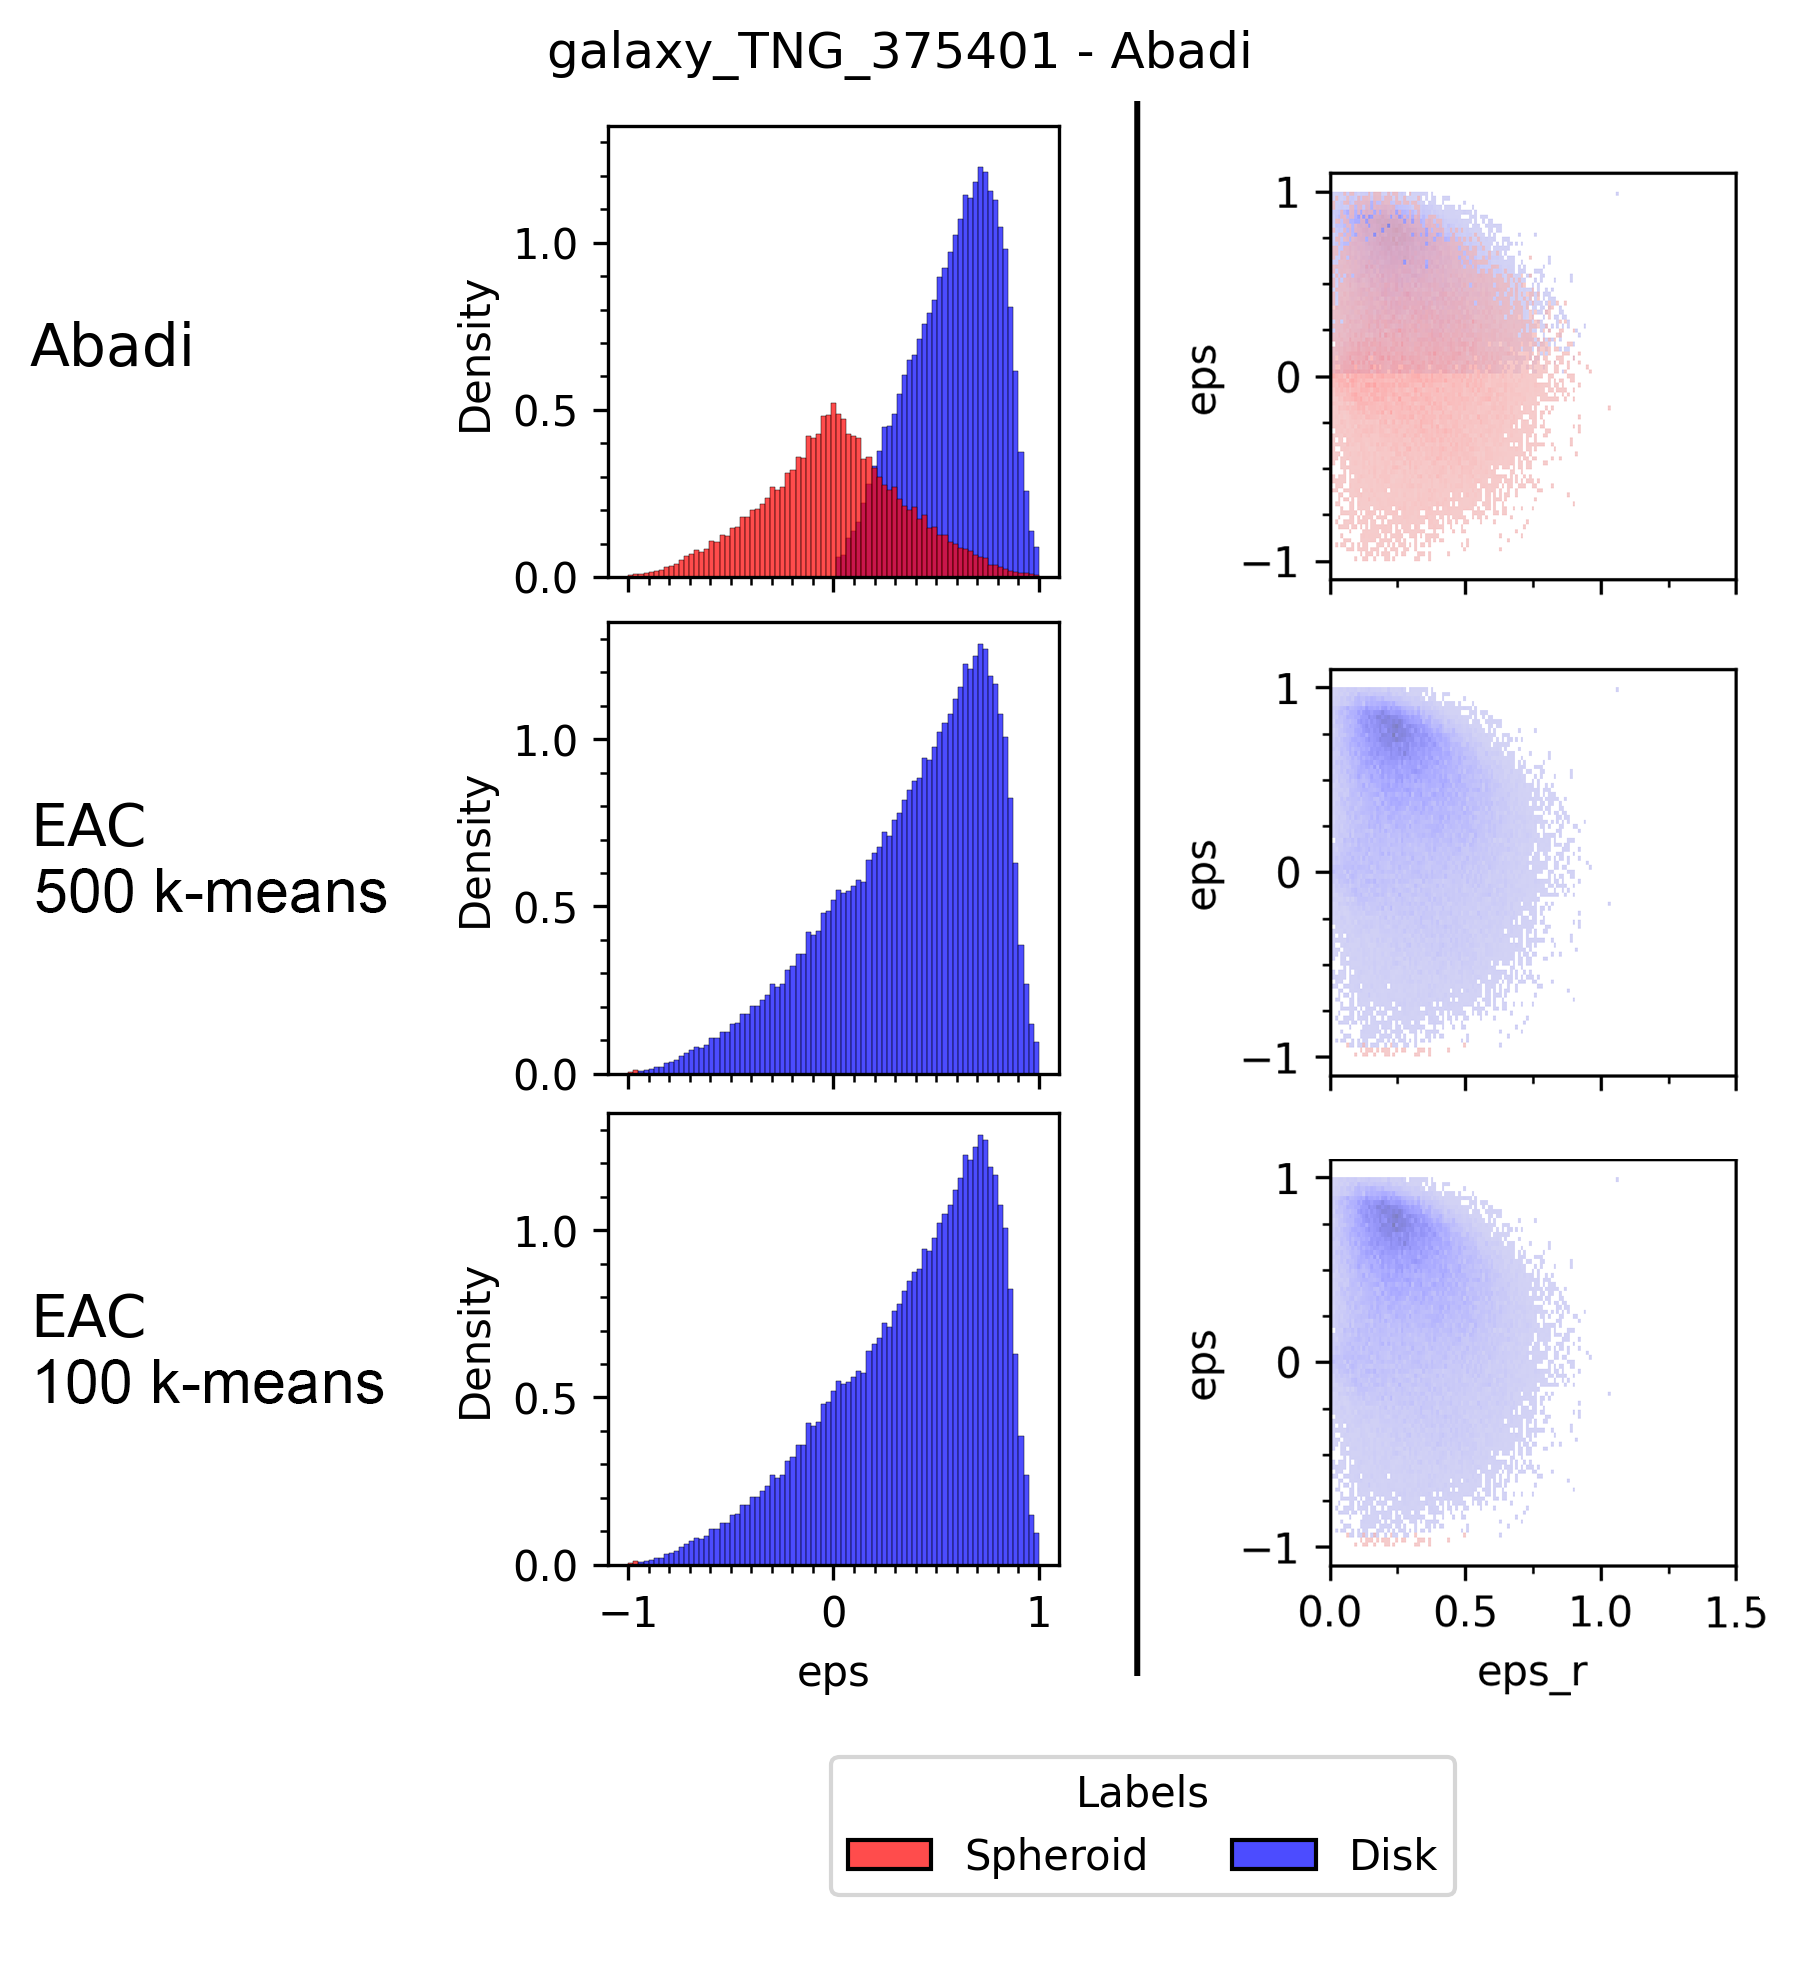
\includegraphics[width=.9\textwidth]{evidence accumulation clustering/figures/eac kmeans 500 vs 100.png}
    \caption{Comparación \gls{EAC} con 500 k-means contra \gls{EAC} con 100 k-means sobre la galaxia \textit{galaxy\_TNG\_375401}.}
    \label{fig:eac-amount-kmeans-comparison}
\end{figure}

Lamentablemente, el costo computacional asociado a utilizar 100 corridas en lugar de 500 sigue siendo alto, lo cual nos impidió realizar todos los experimentos planeados como hicimos en los dos capítulos anteriores en un tiempo razonable. Sin embargo, los resultados que si alcanzamos a obtener con las corridas que hicimos están tan alejados del \gls{GT} que dicha falta de experimentos no son de gran impacto en nuestro análisis.

Como ya se pudo observar en la Fig~\ref{fig:eac-amount-kmeans-comparison}, las clasificaciones obtenidas distan mucho de las reales. En la figura mencionada también se puede apreciar cómo la gran mayoría de las partículas estelares se concentra en uno de los dos clusters. Para entender por qué sucede esto debemos pasar nuestra atención al comportamiento de cada k-means individual aplicado sobre la galaxia.

\begin{figure}
    \centering
    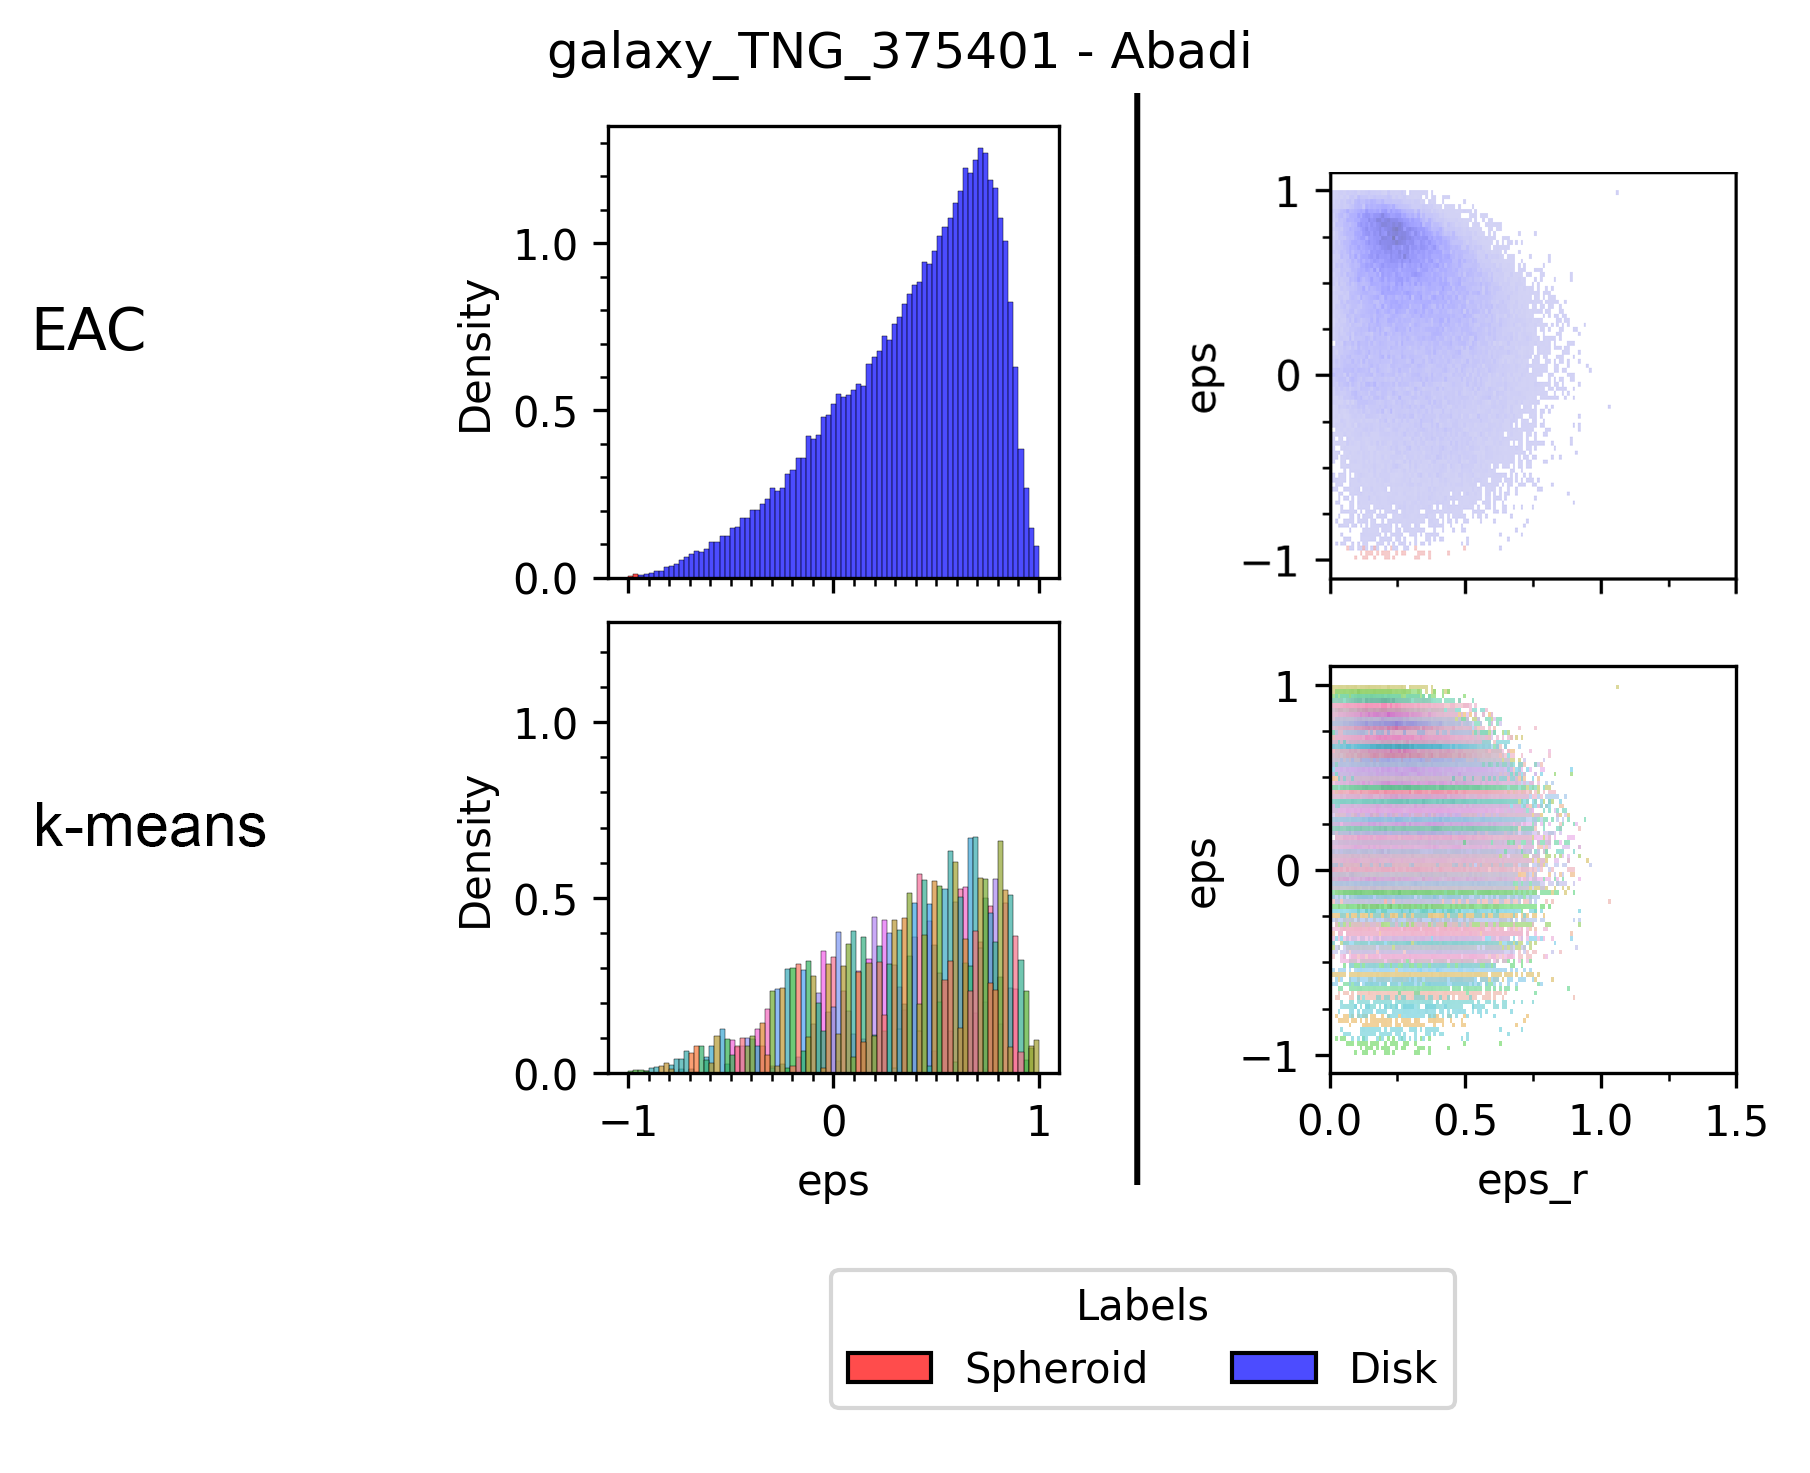
\includegraphics[width=.9\textwidth]{evidence accumulation clustering/figures/kmeans example.png}
    \caption{Comparación \gls{EAC} contra una sola instancia de k-means  sobre la galaxia \textit{galaxy\_TNG\_375401}.}
    \label{fig:eac-single-kmeans-comparison}
\end{figure}

En la Fig~\ref{fig:eac-single-kmeans-comparison} se puede ver cómo los clusters parecen estar separados en líneas siguiendo $eps$. La razón de esto parece ser que, dado que la columna $eps$ es la única fuente de información desde la cual k-means puede derivar clusters, cada partícula estelar será etiquetada con el centro del cluster más cercano en el eje $eps$. Y, de forma similar a como sucedió en el capítulo anterior, esto culmina en clusters divididos por líneas perpendiculares al eje $eps$, ya que no tienen otras columnas o datos desde los cuales derivar clusters y aumentar la dimensionalidad de estas divisiones.

Luego de realizar las 100 corridas diferentes de k-means que aplica \gls{EAC}, dado que la clusterización está siendo realizada sobre un solo eje, a medida que avanza la aglomeración del \gls{HC} que se realiza en el último paso del algoritmo, se irán uniendo clusters adyacentes en el eje $eps$ hasta obtener los últimos dos, separados por una línea recta en dicho eje.

Dado que estamos utilizando single-linkage en el segundo paso de \gls{EAC}, como vimos en el capítulo de Clustering Jerárquico, la métrica de disimilitud entre dos clusters es la menor distancia posible entre dos puntos de ambos. En este caso, el mejor resultado al que el método podía aspirar (dividir verticalmente los datos en $eps$) hubiera requerido que las partículas alrededor del punto donde la densidad del Disco supera a la del Esferoide en Abadi no hayan compartido muchos clusters. Pero, dado lo cercanos que están todos los puntos en $eps$, \gls{EAC} tenderá a priorizar fusionar los clusters que se encuentran en los lugares de mayor densidad del conjunto de datos, ya que al aumentar la densidad de los puntos las probabilidades de encontrar clusters con métricas de disimilitud pequeñas se incrementa al utilizar single-linkage. Es por esto que el Disco encontrado por \gls{EAC} es tan pequeño en comparación al encontrado por Abadi y se encuentra en un extremo de la Fig~\ref{fig:eac-amount-kmeans-comparison}. Alternativamente, podemos ver el mismo efecto en el otro extremo de $eps$ en la Fig~\ref{fig:eac-abadi-469438}.

\begin{figure}
    \centering
    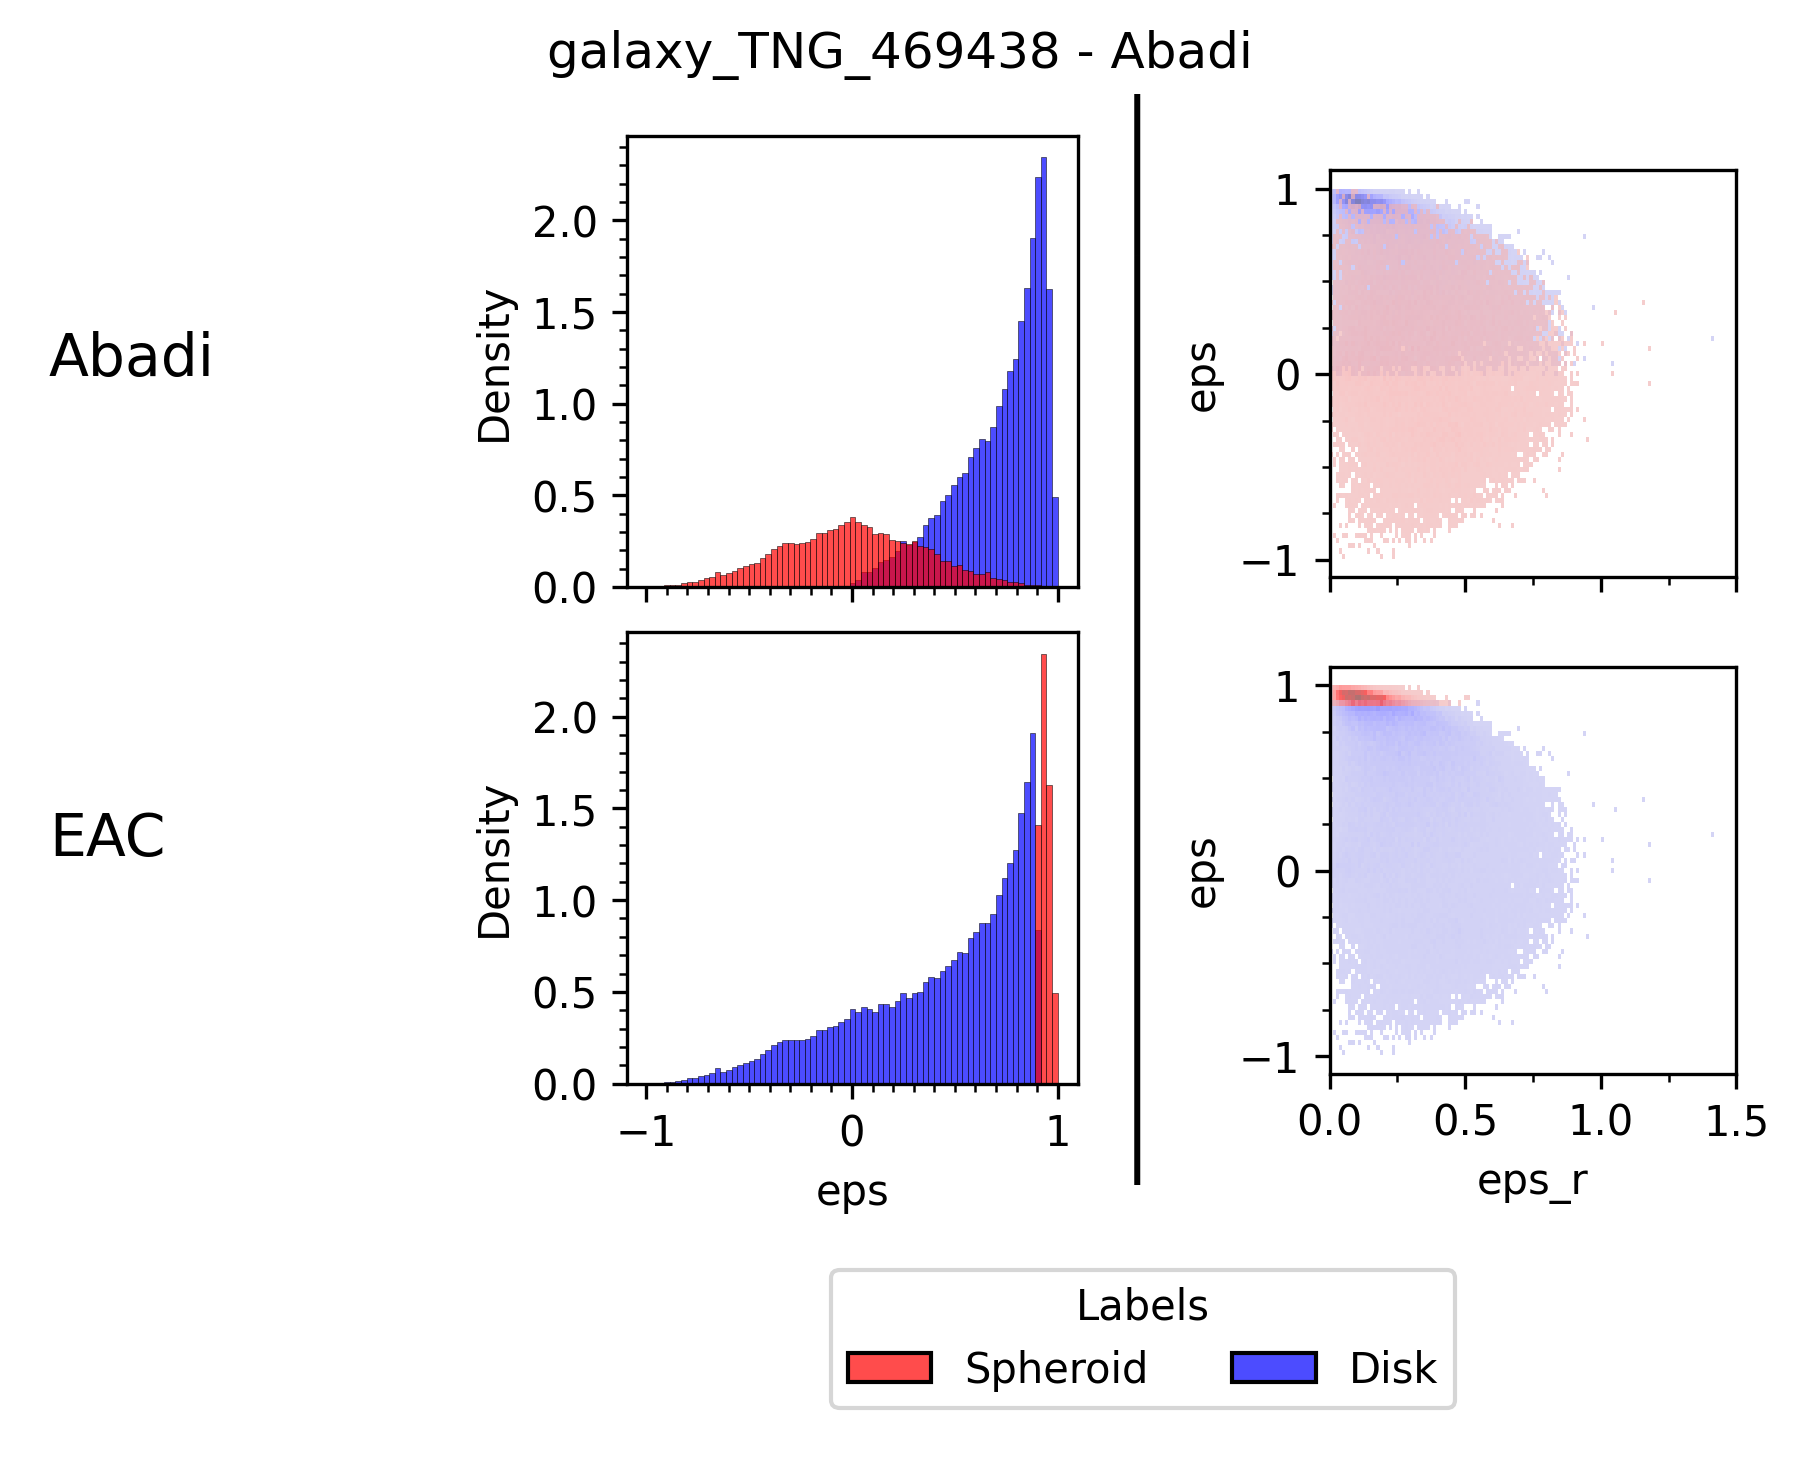
\includegraphics[width=.9\textwidth]{evidence accumulation clustering/figures/galaxy_TNG_469438 - eac -abadi.png}
    \caption{Comparación Abadi contra \gls{EAC} sobre la galaxia \textit{galaxy\_TNG\_469438}.}
    \label{fig:eac-abadi-469438}
\end{figure}

Nuevamente, lo visto en la Fig~\ref{fig:eac-abadi-469438} es resultado de nuestra heurística de calcular la métrica de recall comparando las clasificaciones obtenidas entre \gls{EAC} y Abadi para cada posible combinación de etiquetas en \gls{EAC} y así quedarnos con el conjunto de etiquetas que maximicen el valor de recall. Dado que la diferencia de partículas entre los dos clusters encontrados por \gls{EAC} es tan masiva, la heurística determinó que asignar el cluster encontrado más grande con el cluster de mayor densidad de Abadi era lo más acertado.

Por último, dada la vasta diferencia de los clusters obtenidos con \gls{EAC} comparado con los obtenidos con Abadi y la explicación de por qué sucede esto detallada anteriormente, determinamos que no vale la pena dedicar el tiempo ni el costo computacional necesario para hacer los mismos experimentos eliminando outliers.

Concluimos que \gls{EAC} utilizado con k-means no es una buena alternativa a Abadi, por el costo computacional y de memoria, como así también los resultados deficientes mostrados.

\section{Comparación con Auto Gaussian Mixture - $>$2 clusters}

Nuevamente, utilizamos $N = 100$ para realizar los experimentos con \gls{EAC} y poder comparar sus resultados contra los obtenidos con \gls{AGMM}. Además del alto costo computacional mencionado en la sección anterior, los resultados fueron aún más desalentadores, como puede observarse en la Fig~\ref{fig:eac-agmm-375401}.

\begin{figure}
    \centering
    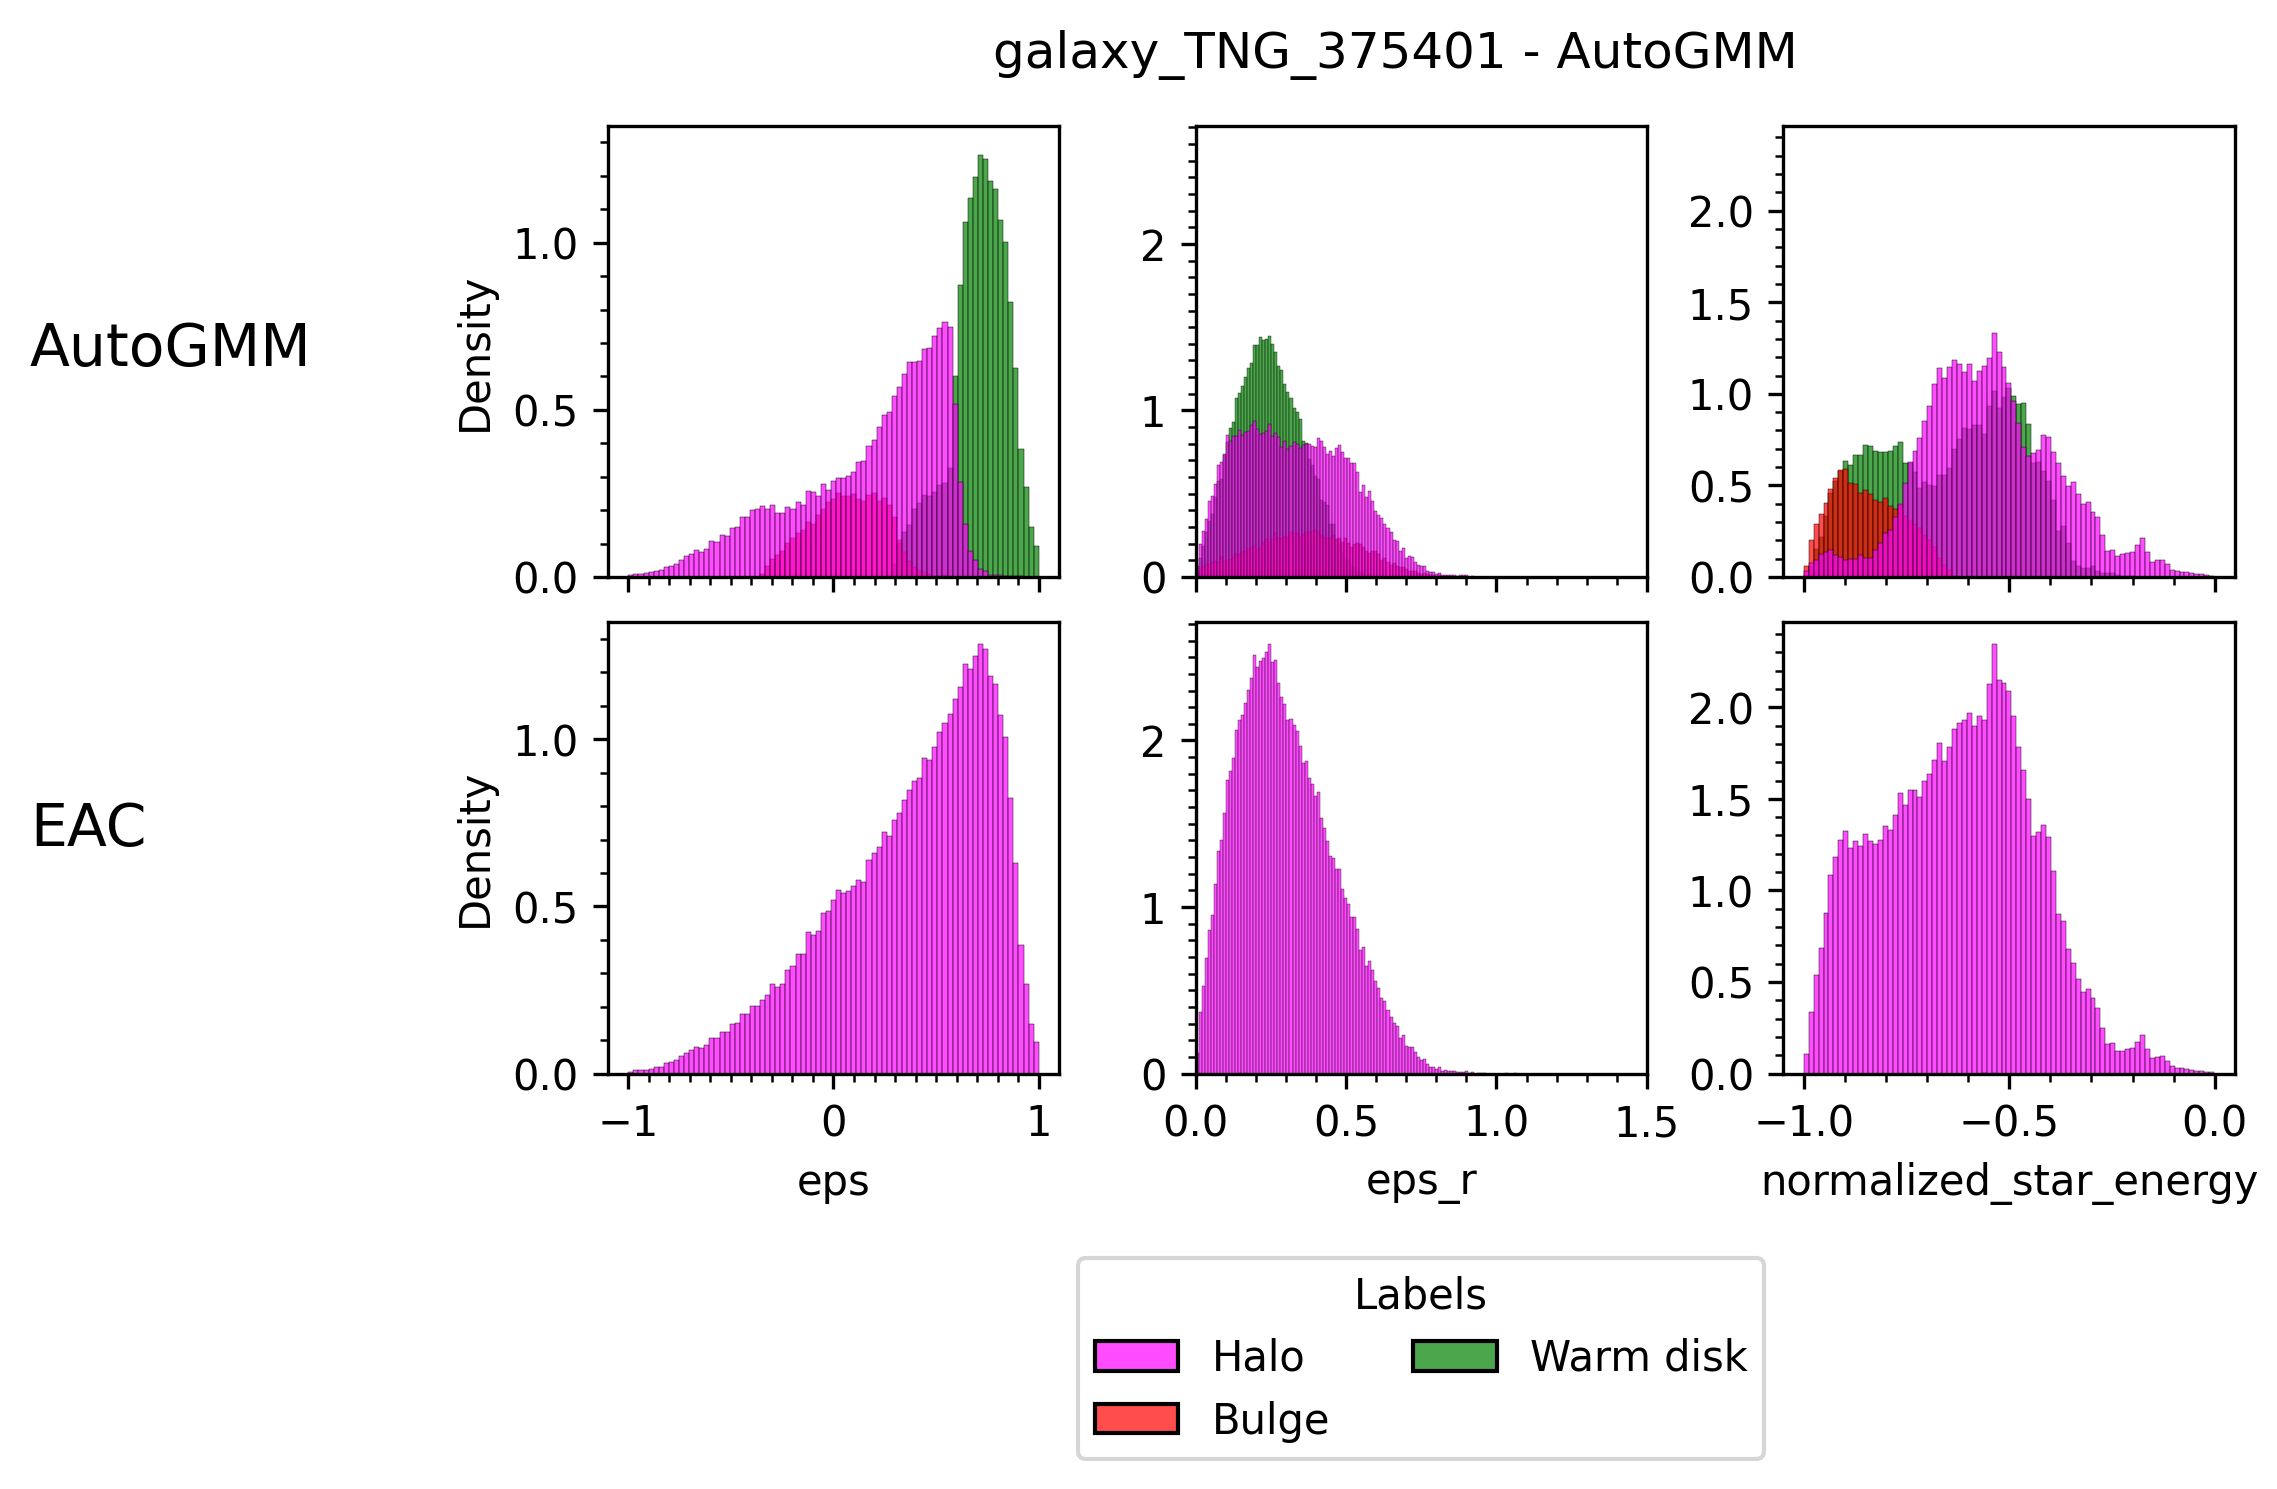
\includegraphics[width=.9\textwidth]{evidence accumulation clustering/figures/galaxy_TNG_375401 - eac - agmm - circ histogram.png}
    \caption{Comparación \gls{AGMM} contra \gls{EAC} sobre la galaxia \textit{galaxy\_TNG\_375401} sobre el histograma del espacio circular.}
    \label{fig:eac-agmm-375401}
\end{figure}

Dado que la limitación sobre las features trabajadas no es un problema en este experimento (ya que utilizamos las tres presentadas al comienzo de este trabajo al tener que comparar contra los resultados obtenidos por \gls{AGMM}), podemos asociar el mal desempeño de \gls{EAC} por el valor de $k$ elegido para los k-means utilizados dentro de éste. Utilizar valores tan altos de $k$ (es decir $k_i = 100, i = 1, ..., N$ como ya habíamos mencionado) puede derivar en una sobre-partición de los k-means, lo que dificulta encontrar los patrones buscados en el dataset. El resultado es una matriz de consenso ruidosa y que no captura correctamente las co-ocurrencias de los puntos.

Potencialmente, como se sugiere en uno de los experimentos realizados en \cite{fred2005combining}, variar los valores de $k$ utilizados por cada k-means (dentro de las cotas adecuadas) en una misma corrida de \gls{EAC} es más robusto que utilizar un $k$ fijo. En dicho trabajo, se argumenta que usar un rango amplio de valores puede llegar a tener un efecto de promediado que nos lleve a la identificación de la estructura verdadera de nuestros datos. Lamentablemente, como bien se explicó en la sección anterior, dados los grandes costos computacionales de aplicar \gls{EAC} sobre nuestro conjunto de datos como así también el tiempo finito que se tuvo para realizar los experimentos, no nos es posible seguir investigando en la dirección sugerida variando el valor de $k$ en cada corrida de k-means, y menos aún poder optimizar las cotas de dicha variación como hiperparámetros.

Finalmente, dados los pésimos resultados obtenidos al buscar más de dos componentes y los altos costos computacionales y de memoria, no nos es posible recomendar \gls{EAC} como alternativa a \gls{AGMM} con las pruebas encontradas hasta el momento.
